\documentclass[12pt,a4paper]{article}


% ==== Packages ====
\usepackage[utf8]{inputenc}
\usepackage[english]{babel}
\usepackage{graphicx}
\usepackage{amsmath}
\usepackage{geometry}
\usepackage{hyperref}
\usepackage{setspace}
\usepackage{titlesec}
\usepackage{fancyhdr}
\usepackage{float}
\usepackage{url}
\usepackage{amsmath, amssymb}
\usepackage{graphicx}
\usepackage{caption}


% ==== Page setup ====
\geometry{margin=1in}
\setstretch{1.3}
\pagestyle{fancy}
\fancyhf{}
\rhead{Linear Discriminant Analysis}
\cfoot{\thepage}
\setlength{\parindent}{0pt}
\setlength{\parskip}{1em}
\newcommand{\HRule}{\rule{\linewidth}{0.5mm}}
% ==== Title formatting ====
\titleformat{\section}{\large\bfseries}{\thesection.}{0.5em}{}
\titleformat{\subsection}{\normalsize\bfseries}{\thesubsection.}{0.5em}{}

% ==== Document ====
\begin{document}
\begin{titlepage}
\centering


\includegraphics[width=0.35\textwidth]{images/program_logo.png}\\[1cm]
{\Large \textbf{D.P.M.S.}\\[0.2cm] Artificial Intelligence}\\[2cm]

\begin{minipage}{0.45\textwidth}
    \centering
    
\includegraphics[height=2.2cm]{images/unipi_logo.png}\\[0.3cm]
    {\small University of Piraeus}
\end{minipage}
\hfill
\begin{minipage}{0.45\textwidth}
    \centering
    
\includegraphics[height=2.2cm]{images/demokritos_logo.png}\\[0.3cm]
    {\small NCSR "Demokritos"}
\end{minipage}

\vspace{2.5cm}

% === Τίτλος Εργασίας ===
\HRule \\[0.6cm]
{\huge \bfseries Linear Discriminant Analysis (LDA)}\\[0.3cm]
\HRule \\[2.5cm]

{\LARGE Theodora Pavlidou}\\[1cm]

\vfill

{\Large
\ifcase\month\or January\or February\or March\or April\or May\or June\or July\or August\or September\or October\or November\or December\fi, \number\year}

\end{titlepage}

\tableofcontents
\newpage

% ==== 1. Introduction ====
\section{Introduction}

Linear Discriminant Analysis (LDA) is a foundational method in data science and machine learning for \textbf{classification and dimensionality reduction}. It identifies linear combinations of features that maximize separation between classes, enhancing the ability to distinguish groups effectively. LDA was developed by \textbf{Ronald A. Fisher in 1936} to classify \textbf{Iris species} based on morphological measurements. Fisher's method established a rigorous statistical framework for multivariate analysis and demonstrated practical utility in distinguishing multiple classes.\par

This report provides a structured exploration of LDA from both theoretical and practical perspectives. Section 2 presents the mathematical foundations of the algorithm, detailing the computation of scatter matrices, the optimization of Fisher’s criterion, and the derivation of linear discriminants. Section 3 describes the preprocessing steps, algorithmic workflow, and implementation considerations necessary for robust application. Section 4 demonstrates LDA in practice using the Iris dataset, illustrating the transformation of data into a lower-dimensional space and the improvement in class separability. Section 5 extends this example by applying a neural network classifier to the LDA-transformed features, highlighting the enhanced performance compared to raw data. Finally, Sections 6 and 7 discuss the limitations, potential enhancements, and future research directions, providing a comprehensive view of LDA’s role in modern machine learning pipelines.\par


% ==== 2. Theoretical Background ====
\section{Theoretical Background and Mathematical Foundation}

Linear Discriminant Analysis (LDA) is a statistical method designed to identify linear combinations of features that optimally separate multiple classes while minimizing within-class variability \cite{fisher1936use}. Rooted in multivariate statistical theory, LDA assumes that the observations for each class follow a multivariate normal distribution with distinct means but a common covariance matrix, a condition known as homoscedasticity \cite{hastie2009elements}. This assumption enables the derivation of linear decision boundaries that maximize class separability.\par

The goal of LDA is to project high-dimensional data into a lower-dimensional space that maximizes the ratio of between-class variance to within-class variance. This is achieved through the use of scatter matrices, which quantify variability within and between classes \cite{duda2001pattern}.For a dataset with $C$ classes, let $\mathbf{X}_k$ denote the set of $n_k$ observations in class $k$, where each observation $\mathbf{x} \in \mathbb{R}^p$.\par

% Mean vectors
Linear Discriminant Analysis (LDA) is a statistical method designed to identify linear combinations of features that optimally distinguish multiple classes while minimizing variability within each class \cite{fisher1936use}. Rooted in multivariate statistical theory, LDA assumes that observations for each class follow a multivariate normal distribution with distinct means but a shared covariance matrix, a condition known as homoscedasticity \cite{hastie2009elements}. This assumption simplifies the derivation of linear decision boundaries, enabling effective separation of classes in the feature space.\par

The objective of LDA is to project high-dimensional data into a lower-dimensional subspace that maximizes the ratio of between-class variance to within-class variance. This process relies on scatter matrices, which quantify the variability within and between classes \cite{duda2001pattern}. For a dataset with $C$ classes, let $\mathbf{X}_k$ denote the set of $n_k$ observations in class $k$, where each observation $\mathbf{x} \in \mathbb{R}^p$ represents a $p$-dimensional feature vector. The following mathematical constructs define the framework for achieving LDA’s goals.\par

The mean vector for class $k$ is computed as:
\[
\boldsymbol{\mu}_k = \frac{1}{n_k} \sum_{\mathbf{x} \in \mathbf{X}_k} \mathbf{x}
\]
This vector represents the centroid of class $k$ in the $p$-dimensional feature space, acting as the ``center of gravity'' for all data points in that class. Physically, it locates the average position of the class. The significance of this centroid lies in its role as a reference point for class identity: classes with widely separated centroids are naturally more distinguishable, while closely spaced centroids indicate a harder classification problem. The mean vector provides a foundation for measuring how far data points deviate within a class and how far class centers are from each other.

The overall mean of all observations across all classes is given by:
\[
\boldsymbol{\mu} = \frac{1}{n} \sum_{k=1}^C \sum_{\mathbf{x} \in \mathbf{X}_k} \mathbf{x}
\]
Here, $n = \sum_{k=1}^C n_k$ is the total number of observations. This vector represents the global centroid of the dataset. Geometrically, it anchors the dataset in the feature space, providing a reference for assessing how far each class’s centroid deviates from the overall average. The physical significance is its role in quantifying the spread of class means: a dataset with class means far from the overall mean suggests greater potential for class separation, as the classes are naturally dispersed across the feature space.

The within-class scatter matrix, which captures the variability of samples around their class means, is defined as:
\[
\mathbf{S}_W = \sum_{k=1}^C \sum_{\mathbf{x} \in \mathbf{X}_k} (\mathbf{x} - \boldsymbol{\mu}_k)(\mathbf{x} - \boldsymbol{\mu}_k)^\top
\]
This matrix quantifies the compactness of each class by measuring how much individual data points deviate from their class centroid. Geometrically, it describes the size and shape of the ``cloud'' of data points within each class. A small $\mathbf{S}_W$ indicates that data points are tightly clustered around their class mean. Physically, this reflects low intra-class variability, which is desirable for LDA, as compact classes are easier to distinguish. The matrix is a sum of outer products, weighted by the number of observations per class.

The between-class scatter matrix, which measures the deviation of class means from the overall mean, is given by:
\[
\mathbf{S}_B = \sum_{k=1}^C n_k (\boldsymbol{\mu}_k - \boldsymbol{\mu})(\boldsymbol{\mu}_k - \boldsymbol{\mu})^\top
\]
This matrix captures the spread of class centroids relative to the dataset’s overall centroid. Physically, it reflects how far apart the classes are in the feature space. A large $\mathbf{S}_B$ indicates that class means are widely dispersed, resembling distinct clusters spread across the feature space. This is critical for LDA, as greater separation between class centroids facilitates better discrimination. Each term in the sum, multiplied by $n_k$, shows how much the class mean's deviation contributes to the overall between-class spread, and the outer product shows the direction and size of this deviation.

The total scatter matrix, representing the overall dispersion of the data, is defined as:
\[
\mathbf{S}_T = \mathbf{S}_W + \mathbf{S}_B
\]
This matrix encapsulates the total variability of the dataset, combining both within-class and between-class scatter. Geometrically, it describes the overall spread of all data points in the feature space, regardless of class labels. While not directly optimized in LDA, $\mathbf{S}_T$ ensures the consistency of the scatter matrix decomposition and reflects the dataset’s global structure.

These illustrations provide a visual understanding of the geometric relationships between the scatter matrices, mean vectors, and the decision boundaries. The following figures depict how the class centers and scatter matrices relate spatially, aiding in the intuitive grasp of how LDA maximizes class separation.\par

\begin{figure}[ht]
    \centering
    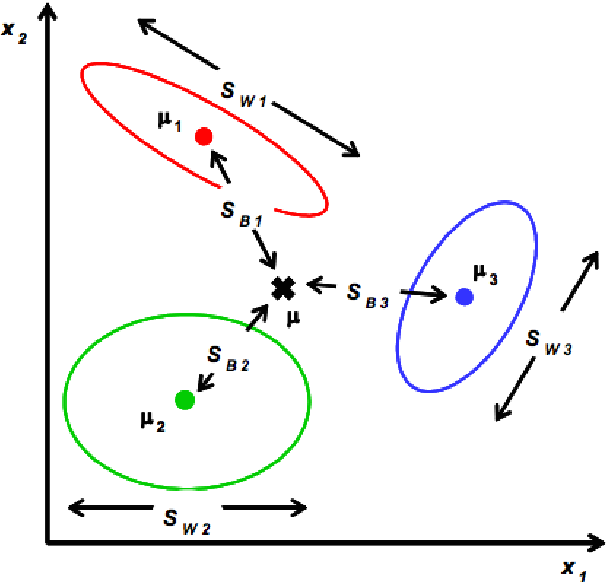
\includegraphics[width=0.5\textwidth]{images/LDA_multi_class.png}
    \caption{Graphical representation of the scatter matrices and the mean vectors ($\boldsymbol{\mu}_k$), variance matrices ($\mathbf{S}_W$, $\mathbf{S}_B$), and the total scatter matrix ($\mathbf{S}_T$). The figure illustrates how the classes differ geometrically and how the decision boundary can be defined via these vectors.~\cite{li2007fisher}}
\end{figure}


\begin{figure}[ht]
    \centering
    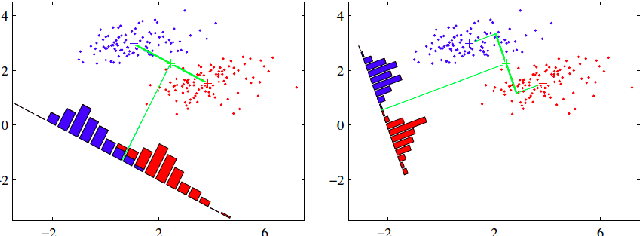
\includegraphics[width=0.8\textwidth]{images/LDA.png} 
    \caption{Example of 2D data points with the directions of Fisher’s linear discriminant ($\mathbf{w}$) and class centroid positions ($\boldsymbol{\mu}_i$). The decision boundary line shows how the optimal separation is achieved through a linear transformation.~\cite{li2007fisher}}
\end{figure}

% Overall explanation
These images help to better visualize the geometric relationships between scatter matrices, mean and variance vectors, and how LDA achieves the optimal class separation. The first image illustrates the geometric elements and their relationships, while the second shows a practical example in two dimensions, emphasizing the role of the Fisher discriminant direction and class centers.

Fisher’s criterion seeks a projection matrix $\mathbf{W} \in \mathbb{R}^{p \times d}$ that maximizes class separation while minimizing intra-class variance:
\[
J(\mathbf{W}) = \frac{|\mathbf{W}^\top \mathbf{S}_B \mathbf{W}|}{|\mathbf{W}^\top \mathbf{S}_W \mathbf{W}|}
\]
This criterion is the heart of LDA’s optimization. The projection matrix $\mathbf{W}$ transforms the data into a lower-dimensional subspace of dimension $d \leq C-1$. The numerator measures the volume of the between-class scatter in the projected space, reflecting how far apart the class means are after projection. The denominator measures the volume of the within-class scatter, indicating how compact the classes remain. Physically, maximizing this ratio means finding a subspace where class centroids are as far apart as possible (large numerator) while keeping each class’s data points tightly clustered (small denominator). Geometrically, this corresponds to stretching the distances between class centers while compressing the spread within each class, resulting in well-separated, compact clusters in the projected space.

In the two-class scenario, the criterion simplifies to finding a single projection vector $\mathbf{w}$:
\[
J(\mathbf{w}) = \frac{\mathbf{w}^\top \mathbf{S}_B \mathbf{w}}{\mathbf{w}^\top \mathbf{S}_W \mathbf{w}}
\]
Here, the goal is to project the data onto a single line (a one-dimensional subspace) that maximizes the separation between the two class means while minimizing the spread within each class along this line. Physically, the numerator represents the squared distance between the projected class means, and the denominator represents the combined variance of the classes along the projection direction. The optimal solution is:
\[
\mathbf{w} \propto \mathbf{S}_W^{-1} (\boldsymbol{\mu}_1 - \boldsymbol{\mu}_2)
\]
This solution defines a direction in the feature space that aligns with the difference between the two class means, adjusted by the inverse of the within-class scatter matrix. The inverse $\mathbf{S}_W^{-1}$ ``normalizes'' the within-class variability, ensuring that the projection direction accounts for the covariance structure. Physically, this direction points along the line that best separates the two class centroids while keeping the projected data points within each class as compact as possible.

For multiple classes, the optimal projection matrix $\mathbf{W}$ is obtained by solving the generalized eigenvalue problem:
\[
\mathbf{S}_B \mathbf{w} = \lambda \mathbf{S}_W \mathbf{w}
\]

This equation finds the directions (eigenvectors) that maximize class separability in the projected space. Each eigenvector $\mathbf{w}$ represents a direction, and its eigenvalue $\lambda$ measures how well the classes are separated along it. The projection matrix $\mathbf{W}$ is formed from the $d \le C-1$ eigenvectors with the largest eigenvalues, creating a low-dimensional subspace where classes are spread apart and overlaps are minimized. The limit $d \le C-1$ exists because the between-class scatter matrix has at most $C-1$ independent directions.

Overall, LDA uses mean vectors to locate class centers, scatter matrices to quantify spread within and between classes, and Fisher’s criterion to find the best projection. These components transform the data into a subspace where classes are compact and well-separated, facilitating classification. The method assumes normally distributed classes with equal covariances, simplifying the geometry, though this may not always hold. \cite{bishop2006pattern}.



% ==== 3. Algorithm Description ====
\section{Preprocessing, Algorithm, and Implementation of Linear Discriminant Analysis}

Linear Discriminant Analysis (LDA) is a statistical method that combines dimensionality reduction with optimal class separation. Its effective use depends on proper data preprocessing and a clear, computationally efficient workflow.

\subsection{Algorithm Description and Implementation Steps}

\textbf{Preprocessing.} Standardize each feature to have zero mean and unit variance to mitigate the impact of differing scales:
\[
\mathbf{x}_j \leftarrow \frac{\mathbf{x}_j - \mu_j}{\sigma_j}
\]
Handle missing values via imputation or exclusion, and remove outliers if necessary. If the number of features $p$ exceeds the number of observations $n$, apply dimensionality reduction (e.g., PCA) to avoid singularity in $\mathbf{S}_W$.

\textbf{Compute class means and overall mean.} For each class $k$, compute:
\[
\boldsymbol{\mu}_k = \frac{1}{n_k} \sum_{\mathbf{x} \in \mathbf{X}_k} \mathbf{x}, \quad
\boldsymbol{\mu} = \frac{1}{n} \sum_{k=1}^C \sum_{\mathbf{x} \in \mathbf{X}_k} \mathbf{x}
\]

\textbf{Compute scatter matrices.} Calculate within-class and between-class scatter matrices:
\[
\mathbf{S}_W = \sum_{k=1}^C \sum_{\mathbf{x} \in \mathbf{X}_k} (\mathbf{x} - \boldsymbol{\mu}_k)(\mathbf{x} - \boldsymbol{\mu}_k)^\top, \quad
\mathbf{S}_B = \sum_{k=1}^C n_k (\boldsymbol{\mu}_k - \boldsymbol{\mu})(\boldsymbol{\mu}_k - \boldsymbol{\mu})^\top
\]
Check that $\mathbf{S}_W$ is invertible; regularization may be applied if necessary.

\textbf{Solve the generalized eigenvalue problem.} Find the projection matrix $\mathbf{W}$:
\[
\mathbf{S}_B \mathbf{w} = \lambda \mathbf{S}_W \mathbf{w}
\]
Select the $d \le C-1$ eigenvectors corresponding to the largest eigenvalues to form $\mathbf{W}$.

\textbf{Project the data.} Transform original data into the lower-dimensional subspace:
\[
\mathbf{z} = \mathbf{W}^\top \mathbf{x}
\]

\textbf{Classification (optional).} Assign a new observation $\mathbf{x}$ to a class using the projected means:
\[
\text{class}(\mathbf{x}) = \arg\min_k \|\mathbf{W}^\top \mathbf{x} - \boldsymbol{\mu}_k^\text{projected}\|
\]
Alternatively, discriminant functions can be used:
\[
\delta_k(\mathbf{x}) = \mathbf{x}^\top \mathbf{S}_W^{-1} \boldsymbol{\mu}_k - \frac{1}{2} \boldsymbol{\mu}_k^\top \mathbf{S}_W^{-1} \boldsymbol{\mu}_k + \log(\pi_k)
\]

\textbf{Implementation considerations.} Use efficient linear algebra libraries (e.g., NumPy, LAPACK). In high-dimensional settings, apply regularization or shrinkage to $\mathbf{S}_W$. Assess robustness via cross-validation, especially if normality or homoscedasticity assumptions are questionable.

\section{Understanding and Practical Uses of LDA}

Linear Discriminant Analysis (LDA) is a powerful technique for dimensionality reduction and supervised classification. Unlike unsupervised methods such as PCA, which maximize overall variance, LDA identifies linear combinations of features that best separate predefined classes. By maximizing the ratio of between-class variance to within-class variance, it ensures that the projections highlight meaningful differences between groups, making the data both easier to visualize and more informative for downstream analysis.

In practice, LDA is widely applied across diverse fields. In face recognition and biometric security, LDA helps differentiate individuals based on facial features, fingerprints, or iris patterns, enhancing identification accuracy in real-world systems. In medical diagnosis, by analyzing clinical measurements, LDA can classify patients into risk groups or detect early signs of diseases, supporting timely intervention. In speech and signal recognition, it reduces feature complexity in audio signals while retaining distinctions between phonemes or spoken words, improving recognition performance. In financial and marketing analytics, LDA can separate customer segments or predict credit risk by identifying patterns in multivariate datasets.

Its strength lies in reducing data complexity while preserving discriminative information, allowing models to train faster and generalize better. Moreover, LDA's results are interpretable, offering insights into which features contribute most to class separation, a critical advantage in regulated or high-stakes domains.

Overall, LDA remains a versatile tool for both exploratory analysis and predictive modeling, and its integration with modern machine learning pipelines continues to enhance the accuracy and robustness of classification systems.

% ==== 4. Practical Example ====
\section{Application Example}
\subsection{LDA on the Iris Dataset}

The \textit{Iris} dataset contains 150 samples of three species (\textit{setosa}, \textit{versicolor}, \textit{virginica}) with four features: sepal length, sepal width, petal length, and petal width. A sample of two rows is shown below:
\begin{table}[h!]
\centering
\begin{tabular}{lcccc}
\hline
Species & Sepal Length & Sepal Width & Petal Length & Petal Width \\
\hline
setosa & 5.1 & 3.5 & 1.4 & 0.2 \\
setosa & 4.9 & 3.0 & 1.4 & 0.2 \\
\hline
\end{tabular}
\end{table}

In the following figure, we can see the feature discriminability ratios for the Iris dataset.

\begin{center}
    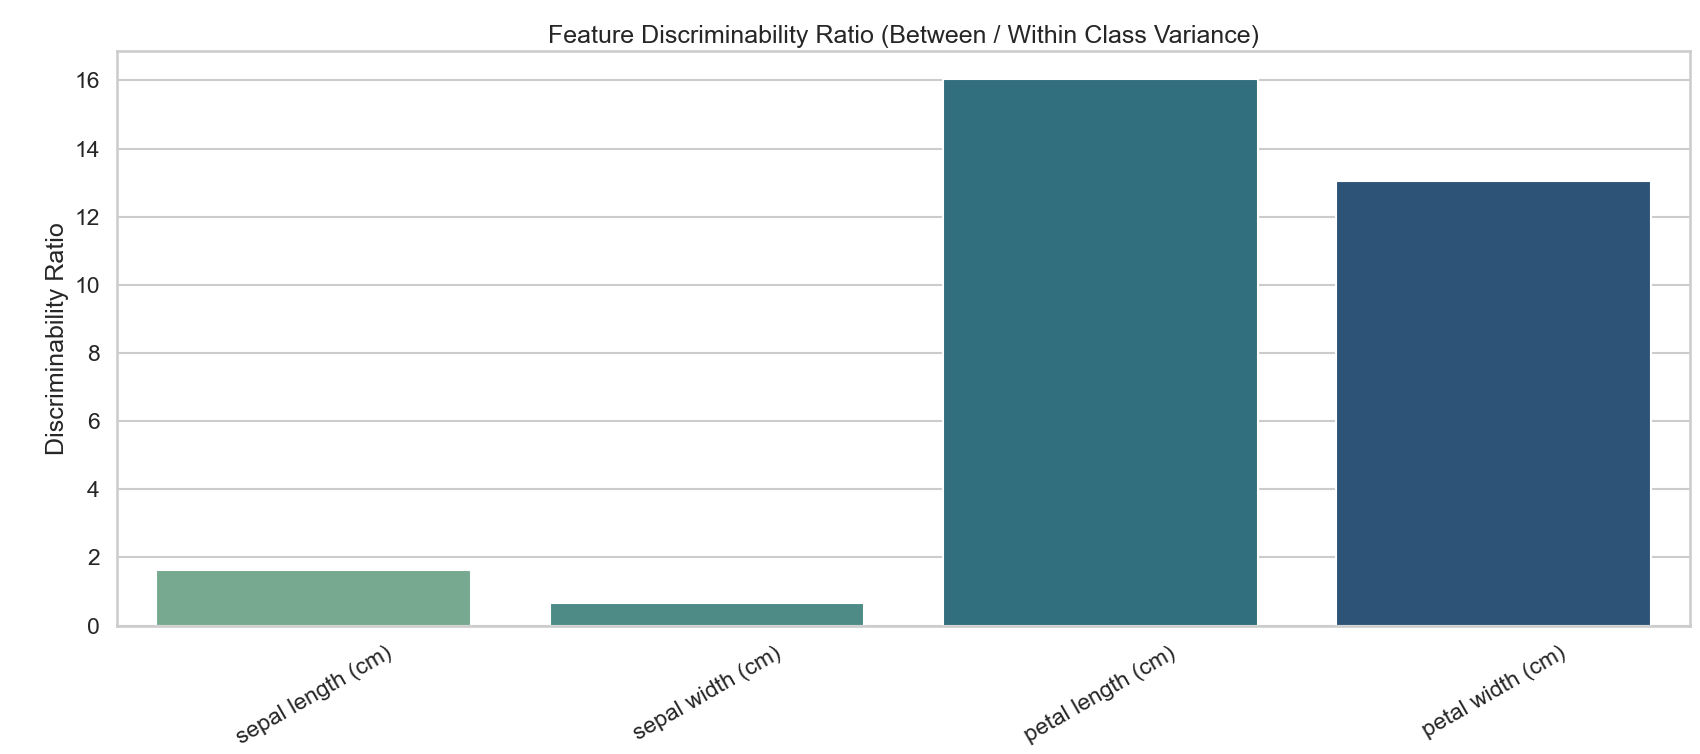
\includegraphics[width=0.7\textwidth]{images/irish_ratio.png}
    \captionof{figure}{Feature discriminability ratios for the Iris dataset.}
\end{center}

In this plot, petal length and petal width clearly separate the species most effectively.

Next, the scree plot shows the amount of discriminative information captured by each linear discriminant.

\begin{center}
    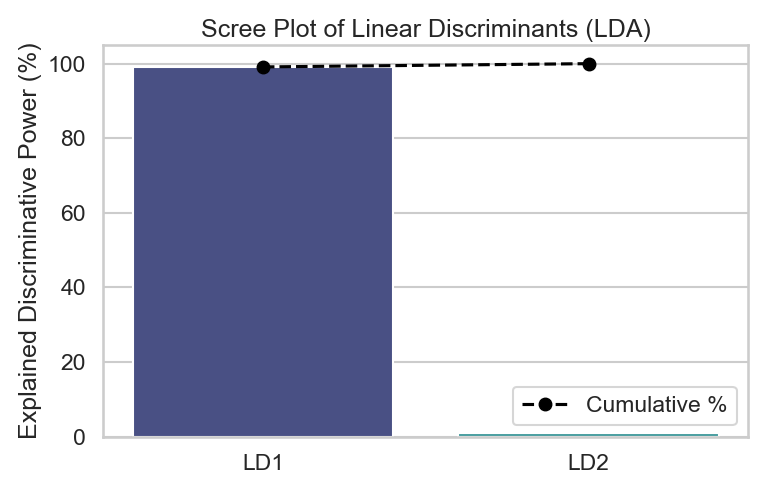
\includegraphics[width=0.7\textwidth]{images/irish_scree_plot.png}
    \captionof{figure}{Scree plot showing the amount of discriminative information captured by each linear discriminant.}
\end{center}

From this diagram, we observe that LD1 captures most of the class separation, while LD2 provides complementary information.

The projection of the Iris data onto the first two linear discriminants is shown in the next figure.

\begin{center}
    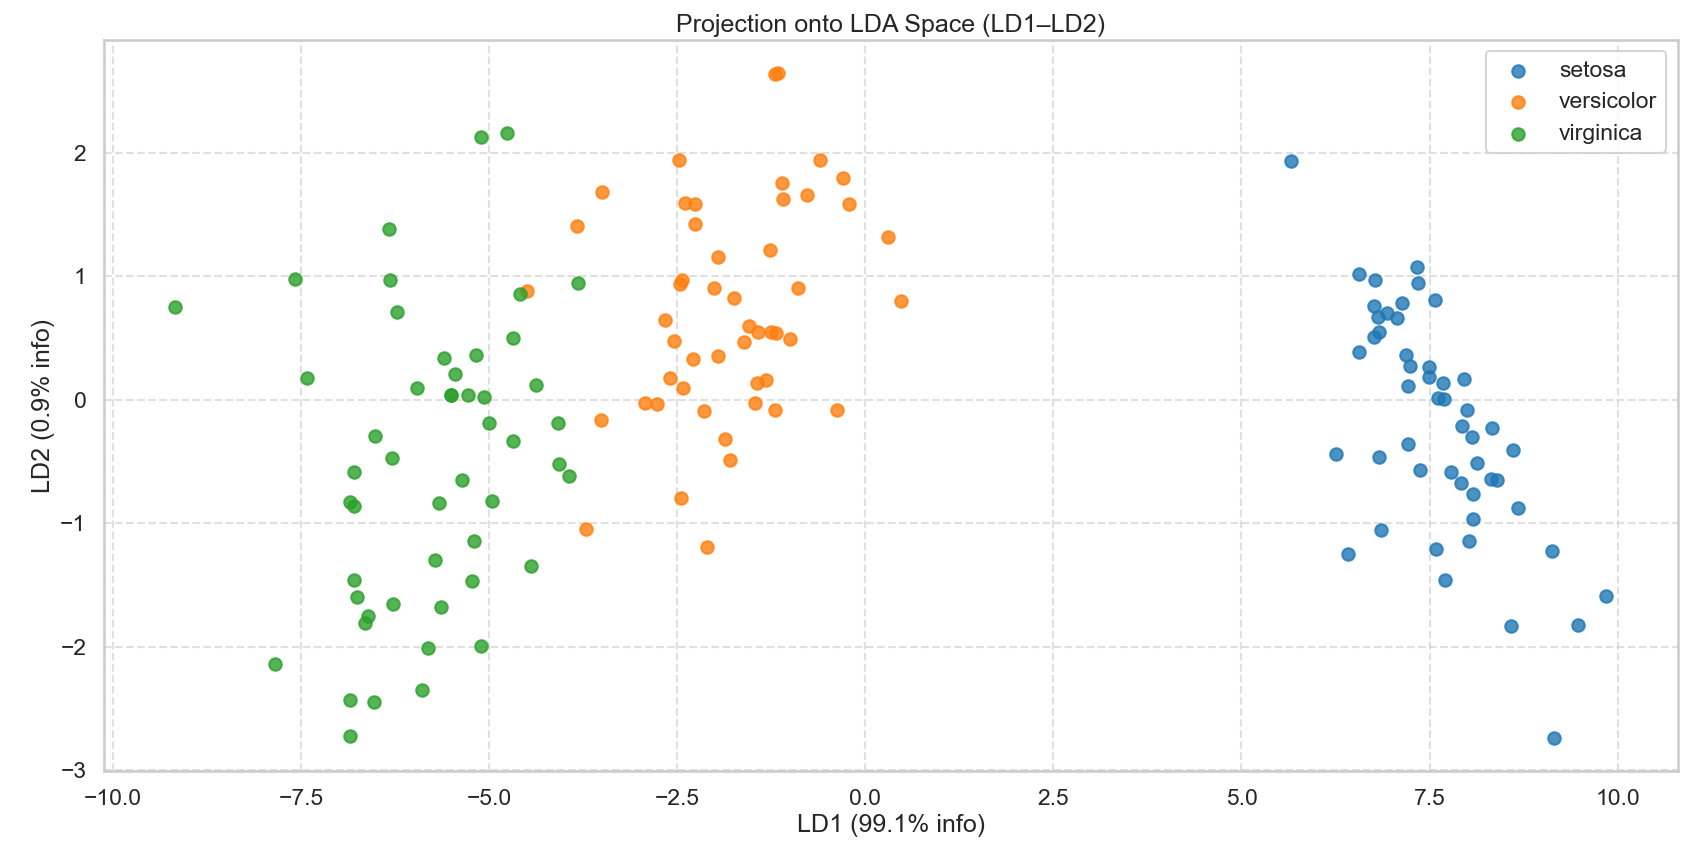
\includegraphics[width=0.7\textwidth]{images/irish_lda.png}
    \captionof{figure}{Projection of the Iris data onto the first two linear discriminants.}
\end{center}

Here, Setosa is clearly separated from the other two species, while Versicolor and Virginica partially overlap along LD2.

Finally, the comparison between the original feature space and the LDA-transformed space is presented below.

\begin{center}
    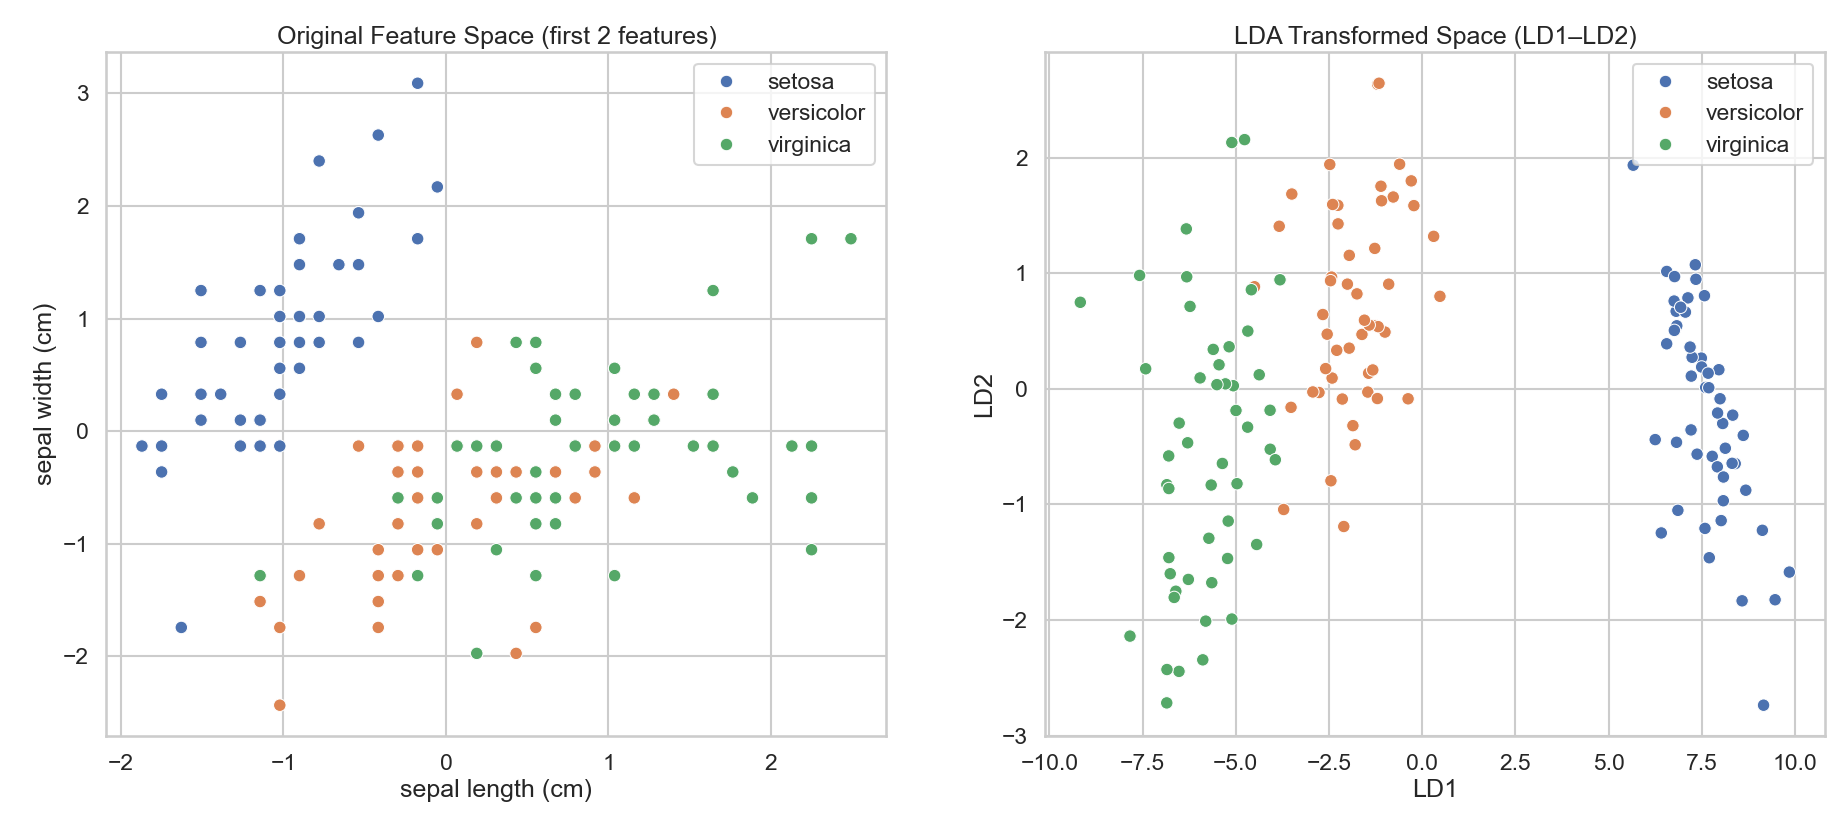
\includegraphics[width=0.7\textwidth]{images/irish_compare.png}
    \captionof{figure}{Comparison between the original feature space and the LDA-transformed space.}
\end{center}

This figure demonstrates that LDA provides a much clearer separation between classes compared to the original feature space.

\subsection{Classification on LDA-Transformed Iris Data}

After transforming the Iris dataset using Linear Discriminant Analysis (LDA), we applied a neural network classifier to evaluate how well the classes can be separated in the reduced feature space. Specifically, we used the \texttt{MLPClassifier} (Multi-Layer Perceptron) from \texttt{scikit-learn}, which is a feedforward artificial neural network capable of learning complex non-linear decision boundaries. The classifier was trained on the LDA-transformed features, which effectively summarize the most discriminative information from the original dataset.

\begin{figure}[h!]
    \centering
    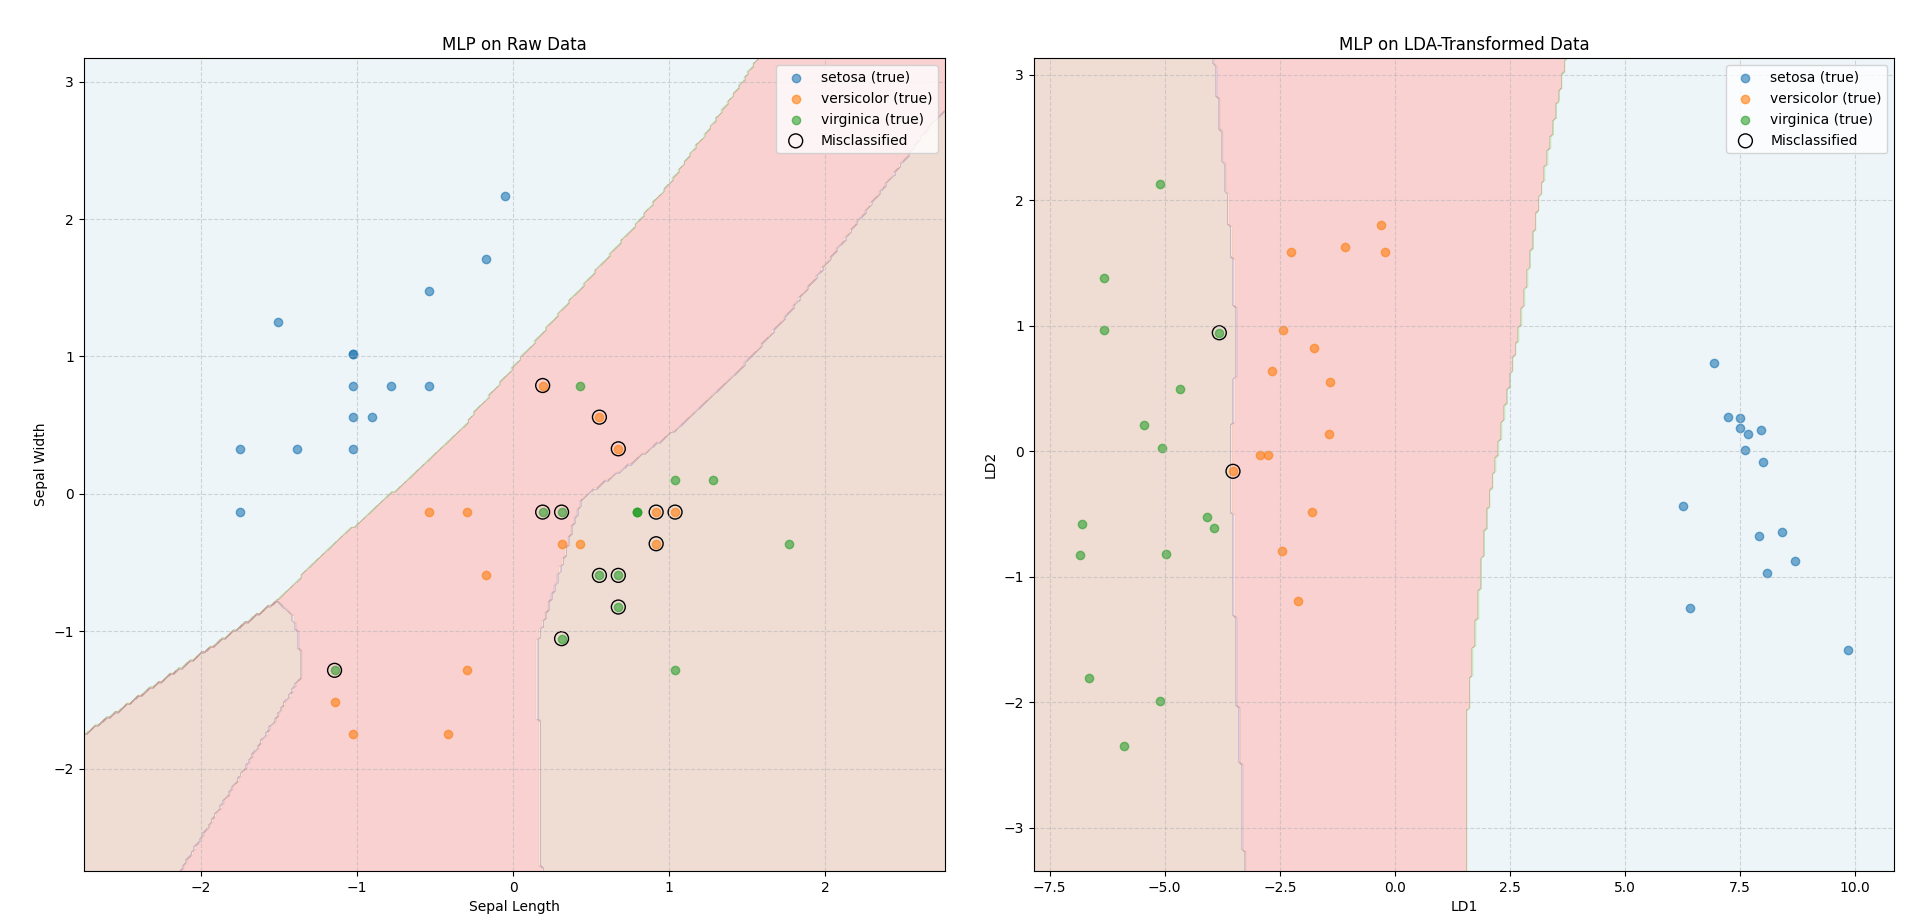
\includegraphics[width=0.7\textwidth]{images/mlp_lda.png}
\end{figure}

In the figure above, each point represents a test sample colored according to its true species, while misclassified points are highlighted with a black circle. The background shading shows the decision regions learned by the MLP classifier. From this visualization, we can see that the MLP is able to separate the species almost perfectly when using the LDA-transformed data. Setosa is completely separated, and Versicolor and Virginica, which partially overlap in the original feature space, are much more distinguishable. This demonstrates the practical value of LDA: by reducing the dimensionality and emphasizing the directions that maximize class separability, it allows a standard classifier like an MLP to perform significantly better than it would on the raw features. In other words, LDA not only simplifies the dataset but also enhances the effectiveness of subsequent machine learning algorithms.

The figures and analysis scripts for this report are available in the repository\footnote{\url{https://github.com/TheodoraPav/LinearDiscriminantAnalysis}}.


\section{Conclusions and Future Work}

Linear Discriminant Analysis (LDA) has proven to be a robust and interpretable technique for dimensionality reduction and classification. By projecting high-dimensional data into a lower-dimensional space that maximizes class separability, LDA provides clear discrimination between groups while reducing the complexity of the data. Its efficiency, simplicity, and ability to handle multiclass problems make it widely applicable across fields such as medical diagnosis, bioinformatics, image recognition, and finance. Furthermore, the linear nature of LDA allows for straightforward interpretation of feature contributions, which is particularly valuable in domains where model transparency is critical.

Future research directions include integrating LDA with advanced machine learning frameworks to improve classification accuracy in high-dimensional or non-linear datasets. Developing robust variants of LDA that can handle imbalanced or noisy data will further enhance its practical applicability. Additionally, exploring hybrid approaches that combine LDA with kernel methods or deep learning architectures may allow it to capture complex, non-linear relationships while preserving the interpretability and efficiency that make LDA a valuable tool. Investigating these avenues will ensure that LDA remains a relevant and effective method in the evolving landscape of data analysis and pattern recognition.


% ==== References ====
\bibliographystyle{plain}
\begin{thebibliography}{10}

\bibitem{fisher1936use}
R.~A. Fisher.
\newblock The use of multiple measurements in taxonomic problems.
\newblock \emph{Annals of Eugenics}, 7(2):179--188, 1936.

\bibitem{hastie2009elements}
T.~Hastie, R.~Tibshirani, and J.~Friedman.
\newblock \emph{The Elements of Statistical Learning: Data Mining, Inference, and Prediction}.
\newblock Springer, 2nd edition, 2009.

\bibitem{duda2001pattern}
R.~O. Duda, P.~E. Hart, and D.~G. Stork.
\newblock \emph{Pattern Classification}.
\newblock Wiley, 2nd edition, 2001.

\bibitem{li2007fisher}
H.~Li.
\newblock Fisher linear discriminant analysis.
\newblock \emph{Online resource, Semantic Scholar}, 2007.
\newblock \url{https://www.semanticscholar.org/paper/Fisher-Linear-Discriminant-Analysis-Li/1ab8ea71fbef3b55b69e142897fadf43b3269463}.

\end{thebibliography}

\end{document}